%!TEX encoding = UTF-8 Unicode
\documentclass[twoside,11pt]{report}
\usepackage[a4paper, total={5.6in, 8.1in}]{geometry}

\usepackage{graphicx}

\usepackage{amssymb, amsmath}
\usepackage[hyperindex,breaklinks,colorlinks,linkcolor=magenta,anchorcolor=blue,citecolor=blue]{hyperref} 
\usepackage{fancyhdr}
\usepackage{floatrow}

\pagestyle{fancy}
\fancyhf{}
\fancyhead[CE]{\footnotesize{\nouppercase\leftmark}}
\fancyhead[CO]{\footnotesize{\nouppercase\rightmark}}
%\fancyhead[RE,LO]{Guides and tutorials}
%\fancyfoot[CE,CO]{\leftmark}
\fancyhead[LE,RO]{\thepage}
\renewcommand{\headrulewidth}{0pt}
\usepackage{etoolbox}
\makeatletter
%\ patchcmd{<cmd>}{<search>}{<replace>}{<success>}{<failure>}
\patchcmd{\chaptermark}{\@chapapp\ }{}{}{}
\makeatother

\usepackage{titlesec}

\makeatletter
\def\@makechapterhead#1{%
  {\parindent \z@ \raggedright \normalfont
    \ifnum \c@secnumdepth >\m@ne
        {\fontsize{19pt}{25pt}\bfseries \thechapter.\ % <-- Chapter # (without "Chapter")
    \fi
    \interlinepenalty\@M
    #1\par\nobreak% <------------------ Chapter title
    \vskip 100\p@% <------------------ Space between chapter title and first paragraph
  }}}
\makeatother


\def\be{\begin{equation}}
\def\ee{\end{equation}}
\def\ii{\text{i}}
\def\dd{\text{d}}
\def\dt{\text{d}t}

\makeatletter % `@' now normal 'letter'
\@addtoreset{equation}{subsection}

\renewcommand\theequation{{\thesection}%
.{\arabic{equation}}}

\usepackage{bm}

\usepackage[utf8]{inputenc}
\usepackage[T1]{fontenc}
%\usepackage[ngerman]{babel}

\allowdisplaybreaks

\usepackage{setspace} 



\title{Quantum Field Theory in Condensed Matter Physics}
\author{Naoto Nagaosa}

\begin{document}
\maketitle
\tableofcontents
\setcounter{page}{0}
\setstretch{1.03}

%!TEX root = ./main.tex

\chapter[Review of Quantum Mechanics and Basic Principles of Field Theory]{Review of Quantum Mechanics and \\ Basic Principles of Field Theory}
The content of this chapter is nothing but a review of the most basic principles. Starting with the quantum mechanics of a single-particle system, then the canonical conjugate relations, the relation between symmetries and conservation laws, the description of multi-particles systems using field theory, finally gauge invariance and the gauge field will be introduced, all begin fundamental concepts that built the basis for the whole following discussion. The reader should reconfirm the universality of the quantum mechanical description and get a taste of the efficiency of an analogy. 


%!TEX root = ./main.tex

\section{Single-Particle Quantum Mechanics}

We start by recalling some facts about single-particle quantum mechanics. All points that will be mentioned here will again become important when proceeding to quantum field theory. 

The equation of motion of the single-particle system is given by the\!\! {\color{white}{\-}}Schrödinger equation:

\be\label{eq1.1.1}
\ii\hbar\frac{\partial\psi({\bm r},t)}{\partial t}=\hat{H}\psi({\bm r},t)=\left[\frac{\hat{\bm p}^2}{2m}+V(\hat{\bm r})\right]\psi({\bm r},t)
\ee
$\psi({\bm r},t)$ is the so-called wave function, depending on the space coordinates $\bm r$ and the time $t$. $\hat H$ is the so-called Hamiltonian operator, creating a new wave function $\hat H\psi({\bm r},t)$ by acting on the wave function $\psi({\bm r},t)$. In what follows, operators are assigned by a hat, except for obvious cases where this notation will be omitted. $\hat{\bm p}$ and $\hat{\bm r}$ are three-component vector operators that represent the \,momentum \,and \,space \,coordinate \,of \,the \,particle, \,respectively. ${\hat{\bm p}}^2/2m$ \-
is the kinetic energy, $V(\hat{\bm r})$ the potential energy, and its sum is the total energy of the particle, called the Hamiltonian operator $\hat H$. Equation \eqref{eq1.1.1} signifies that the time development of the wave function is determined by the Hamiltonian operator $\hat H$. By defining the exponential $\exp(\hat A)$ pf an operator by

\be\label{eq1.1.2}
\exp(\hat A)=\sum_{n=0}^\infty \frac{1}{n!}(\hat A)^n
\ee
its solution can be written as
\be\label{eq1.1.3}
\psi({\bm r},t)\exp\left(-\frac{i}{\hbar}\hat Ht\right)\psi({\bm r},0)
\ee

In quantum mechanics, the wave function is interpreted in terms of probability. The square of the absolute value of the wave function
\be
P({\bm r},t)=|\psi({\bm r},t)|^2
\ee
is interpreted as the probability of detecting the particle at time $t$ at the coordinate $\bm r$. Therefore, because the sum (integral) of the probability over the whole space is $1$, we obtain the normalization condition of the wave function:
\be
\int\dd^3{\bm r}P({\bm r},t)=\int\dd^3{\bm r}|\psi({\bm r},t)|^2=1
\ee

We will now explain the matrix formulation of quantum mechanics. We interpret the function $f({\bm r})$ as a vector in the Hilbert space (the vector space of function) and write $|f\rangle$ for the state that the function represents. Doing so, the operator $\hat A$ acting \,on \,the \,vectors \,in \,this space generates \,a \,new vec\-- \,tor, which is a linear transformation. Therefore, it corresponds to a matrix. 
Furthermore, to every vector $|f\rangle$, there exists the conjugate vector $\langle f|$, being specified as the so-called ket- and bra-vector, respectively. Thinking in components, the bra-vector $\langle f|$ can be regarded as the transposed and complex conjugate of the ket-vector $|f\rangle$. The inner product $\langle g\,|\,f\rangle$ in this vector space is defined by
\be\label{eq1.1.6}
\langle g|f\rangle - \int \dd^3{\bm r}g^*({\bm r})f({\bm r})=\langle f|g\rangle^*
\ee
The matrix element $\langle g|\hat A|f\rangle$ of the operator (the matrix) $\hat A$ is given by
\be\label{eq1.1.7}
\langle g|\hat A|f\rangle = \langle g|\hat Af\rangle = \int \dd^3{\bm r}g^*(r)\hat Af({\bm r})
\ee
In order to give a more concrete picture of the considerations made so far, we introduce now an orthonormal basis $|i\rangle, i=1,2,3\cdots,$ of the Hilbert space. (We wrote $i=1,2,3\cdots;$ however, the basis is not necessarily a countable set. In general, when the volume of the system is infinite, the set of basis vectors is uncountable. In these cases, the sum $\sum_i$ over the set labelled by $i$ must be replaced by an integral. ) Because the basis is orthonormal, the orthonormality condition
\be
\langle i|j\rangle=\delta_{i,j}
\ee
and the completeness condition
\be
\sum_i|i\rangle\langle i|=\hat 1
\ee
hold. Here, the so-called Kronecker delta $\delta_{i,j}$ is defined to equal $1$ when $i=j$, and to be zero otherwise. $\hat 1$ is the identity matrix; in other words, the identity operator. In this basis, the vector $|f\rangle$ can be represented by its components:

\be
|f\rangle = \sum_i|i\rangle\langle i|f\rangle,\quad \langle f|=\sum_i\langle f|i\rangle\langle i|.
\ee
Furthermore, the component representation of $\hat A|f\rangle$ is given by

\be\begin{split}
\hat A|f\rangle &= \left(\sum)i|i\rangle\langle i|\right)\hat A\left(\sum)j|j\rangle\langle j|\right)|f\rangle\\
&=\sum_{i,j}|i\rangle\langle i|\hat A|j\rangle\langle j|f\rangle
\end{split}\ee
and \eqref{eq1.1.7} can be written as

\be
\langle g|\hat A|f\rangle = \sum_{i,j}\langle g|i\rangle\langle i|\hat A|j\rangle\langle j|f\rangle
\ee
We define the Hermitian conjugate $\hat{A}^\dagger$ of $\hat A$ by requiring that

\be\label{eq1.1.13}
\langle g|\hat A|f\rangle = \langle\hat{A}^\dagger g|f\rangle
\ee
holds for every $|f\rangle$ and $|g\rangle$. Comparing the inner product of the conjugate of 
\be
|\hat{A}^\dagger g\rangle = \sum_{j,i}|j\rangle\langle|\hat{A}^\dagger|i\rangle\langle i|g\rangle
\ee
with $|f\rangle$ and

\be
\langle\hat{A}^\dagger g|f\rangle = \sum_{j,i}\langle g|i\rangle\langle j|\hat{A}^\dagger|i\rangle^*\langle j|f\rangle
\ee
with \eqref{eq1.1.13}, we obtain
\be
\langle j|\hat{A}^\dagger|i\rangle = \langle i|\hat A|j\rangle^*
\ee

This is nothing but the usual definition of the Hermitian conjugation of a matrix. In the case that $\hat A$ and $\hat{A}^\dagger$ are equal $\hat A = \hat{A}^\dagger$, $\hat A$ is called a Hermitian operator. In quantum mechanics, all physical quantities are represented in terms of Hermitian operators. 

We now introduce the eigenvalue $a$ and the eigenstate $|a\rangle$ of the Hermitian operator $\hat A$:
\be
\hat A|a\rangle = a|a\rangle
\ee
By taking the inner product with $|a\rangle$
\be
\langle a|\hat A|a\rangle = a\langle a|a\rangle
\ee
we can deduce that at the left-hand side due to hermiticity 

\be\label{eq1.1.19}
\langle a|\hat A|a\rangle = \langle \hat{A}^\dagger a|a\rangle = \langle\hat{A}a|a\rangle - a^*\langle a|a\rangle
\ee
holds, and obtain $a=a*$. Therefore, we conclude that the eigenvalue $a$ is real. Furthermore, for $a\neq a'$ with

\be
\langle a'|\hat A=a'\langle a'|
\ee
from \eqref{eq1.1.19} we can deduce that

\be
\langle a'|\hat A|a\rangle = a\langle a'|a\rangle = a'\langle a'|a\rangle
\ee
and conclude that $\langle a'\, |\, a\rangle = 0$. This signifies that the eigenstates of a Hermitian operator with different eigenvalues are orthogonal to each other. Therefore, by a suitable normalization it is possible to build an orthonormal basis using the eigenstates of an Hermitian operator by orthogonalizing in eigenspaces belonging to the same eigenvalue. 

Naturally, the space coordinate $\hat{\bm r}$ is a Hermitian operator. Every component $\hat{r}_\alpha$ of $\hat{\bm r}$ acts on $f(\hat{\bm r})$

\be\label{eq1.1.22}
\hat{r}_\alpha f({\bm r})=r_\alpha f({\bm r})
\ee
creating a new function. Notice that on the right hand side, $r_\alpha$ is no longer an operator, but the $\alpha$-component of the function $\bm r$. The generalization of \eqref{eq1.1.22} is

\be
V(\hat{\bm r})f({\bm r})=V({\bm r})f({\bm r})
\ee
with $V(\hat{\bm r})$ being the potential energy of equation \eqref{eq1.1.1}. With \eqref{eq1.1.22} we write

\be\begin{split}
\langle g|\hat{r}_\alpha|f\rangle &=\int\dd^3{\bm r}g^*({\bm r})\hat{r}_\alpha f({\bm r})=\int \dd^3g^*({\bm r})r_\alpha f({\bm r})=\int\dd^3{\bm r}[r_\alpha g({\bm r})]^*f({\bm r})\\
&=\int\dd^3{\bm r}[\hat{r}_\alpha g({\bm r})]^*f({\bm r})=\langle\hat{r}_\alpha g|f\rangle
\end{split}\ee
It should be clear from these equations that $\hat{r}_\alpha$ is Hermitian. 

We introduce now the state $|\bm r\rangle$ being the eigenstate with eigenvalue $\bm r$ of the operator $\hat{\bm r}$:

\be
\hat{\bm r}|\bm r\rangle = \bm r|\bm r\rangle
\ee
Because $\langle \bm r'|\bm r\rangle = 0$ for $\bm r\neq\bm r'$, 
\be\label{eq1.1.26}
\langle \bm r'|\bm r\rangle = \delta(\bm r-\bm r')
\ee
with an appropriate choice of the normalization. Here we have introduced the so-called delta function $\delta(\bm r-\bm r')$, defined to be zero for $\bm r\neq\bm r'$, and infinite at $\bm r=\bm r'$, and to give the value $1$ when integrated over $\bm r-\bm r'$ in a region containing the origin. Furthermore, $|\bm r\rangle$ and $\langle\bm r|$ fulfill the completeness relation

\be\label{eq1.1.27}
\int\dd^3\bm r|\bm r\rangle\langle \bm r|=\hat 1
\ee
The reader not familiar with the delta function is referred to the Appendices A and B. As mentioned there, we can introduce a vector space on a discrete lattice. The components of a vector in this space are defined by the values of a function on the discrete lattice points. This vector space approaches the Hilbert space when the number of lattice points $N_L$ becomes infinite, that is, when the lattice spacing $\Delta x$ becomes zero. In this case, the sum $(\Delta x)^3\sum_{\text{lattice points }i}$ approaches the three-dimensional integral appearing in \eqref{eq1.1.6}. As a basis of the $N_L$-dimensional vector space, we define states that are zero at all lattice points except for the coordinate ${\bm r}_i$, where the value is defined to be $1/(\Delta)^{3/2}$. Then we have

\[\langle {\bm r}_i|{\bm r}_j\rangle = \sum_k\frac{\delta_{{\bm r}_i,{\bm r}_k}}{(\Delta x)^{3/2}}\frac{\delta_{{\bm r}_k,{\bm r}_j}}{(\Delta x)^{3/2}}=\frac{\delta_{{\bm r}_i,{\bm r}_j}}{(\Delta x)^{3}}\]
and, furthermore, 
\[(\Delta)^3\sum_i|{\bm r}_i\rangle\langle {\bm r}_i|=\hat{1} \]
In the limit as $\Delta x\to0$, these equations approach the equations of the inner product and the completeness relation of the basis ${\bm r}$ mentioned above. 

Now, owing to the completeness relation of the basis ${\bm r}$, we can write the inner product \eqref{eq1.1.6} as

\be
\langle g|f\rangle = \int\dd^3{\bm r}\langle g|{\bm r}\rangle\langle{\bm r}|f\rangle
\ee
and obtain

\be\begin{split}
f({\bm r})&=\langle{\bm r}|f\rangle,\\
g^*({\bm r})=\langle g|\bm r\rangle.
\end{split}\ee
From this point of view, the wave function $\psi({\bm r},t)$ is nothing but the $\bm r$-component of the state vector $|\psi(t)\rangle$ of the Hilbert space written in the basis $|\bm r\rangle$. 

Now, what about the momentum operator $\hat{\bm p}$? Here, we meet the very first example of the most fundamental relation in quantum mechanics, namely the canonical conjugate relation. A plane wave with wave number $\bm k$ can be expressed as $\psi_{\bm k}({\bm r})=(2\pi\hbar)^{-3/2}e^{i\bm{kr}}$. Writing the place wave as a function of $\bm r$, and using
\be\label{eq1.1.30}
\hat{\bm p}=\frac{\hbar}{\ii}\frac{\partial}{\partial {\bm r}}
\ee
we obtain
\be\label{eq1.1.31}
\hat{\bm p}\psi_{\bm k}({\bm r})=\hbar\bm{k}\psi_{\bm k}(\bm r)=\bm p\psi_{\bm k}(\bm r)
\ee
and therefore the relation $\bm{p=\hbar k}$. We now define the following combination of $\hat{\bm r}$ and $\hat{\bm p}$:
\be
[\hat{r}_\alpha,\hat{p}_\beta]=\hat{r}_\alpha\hat{p}_\beta-\hat{p}_\beta\hat{r}_\alpha
\ee
This is the so-called commutator of $\hat{\bm r}_\alpha$ and $\hat{\bm p}_\alpha$, which is also an operator. Acting with this commutator on an arbitrary function $f({\bm r})$, we obtain
\[\begin{split}
[\hat{r}_\alpha,\hat{p}_\beta]f({\bm r})&=\left(\hat{r}_\alpha\frac{\hbar}{\ii}\frac{\partial}{\partial r_\beta}-\frac{\hbar}{\ii}\frac{\partial}{\partial r_\beta}\hat{r}_\alpha\right)f(\bm r)\\
&=\frac{\hbar}{\ii}\left\{r_\alpha\frac{\partial f(\bm r)}{\partial r_\beta}-\frac{\partial}{\partial r_\beta}(r_\alpha f(\bm r))\right\}
\end{split} \]
and therefore the identity
\be\label{eq1.1.33}
[\hat{r}_\alpha,\hat{p}_\beta]=\ii\hbar\delta_{\alpha,\beta}
\ee
This is the so-called commutation relation. It follows from \eqref{eq1.1.33} for $\alpha=\beta$ that $[\hat{r}_\alpha,\hat{p}_\alpha]=\ii\hbar$. This means that $\hat{r}_\alpha$ and $\hat{p}_\alpha$ are canonical conjugates of each other. This commutation relation, as well as \eqref{eq1.1.30}, is the starting point for many very fundamental and wide conceptual developments that will be discussed in what follow. However, we first discuss some aspects of the eigenstates of $\hat{\bm p}$. We can interpret \eqref{eq1.1.31} as
\be
\hat{\bm p}|\bm p\rangle = \bm p|\bm p\rangle
\ee
\be
\langle\bm r|\bm p\rangle = \psi_{\bm p/\hbar}(\bm r)\frac{1}{(2\pi\hbar)^{3/2}}\exp\left(\frac{\ii}{\hbar}\bm p\cdot\bm r\right)
\ee
$|\bm p\rangle$ also spans a basis; orthogonality can be shown with
\be\label{eq1.1.36}\begin{split}
\langle\bm p'|\bm p\rangle&=\int\dd^3\bm r\langle\bm p'|\bm r\rangle\langle\bm r|\bm p\rangle\\
&=\int\frac{\dd^3\bm r}{(2\pi\hbar)^2}\exp\left[\frac{\ii}{\hbar}(-\bm p'+\bm p)\cdot\bm r\right]=\delta(\bm p-\bm p')
\end{split}\ee
and, in the same manner, the completeness relation
\be\label{eq1.1.37}
\int\dd^3\bm p|\bm p\rangle\langle\bm p|=\hat{1}
\ee
by acting on it with $\langle\bm r'|$ and $|\bm r\rangle$ on the left- and right-hand sides:
\be\begin{split}
\int\dd^3\bm p\langle\bm r'|\bm p\rangle\langle\bm p|\bm r\rangle&=\int\frac{\dd^3\bm p}{(2\pi\hbar)^3}\exp\left[\frac{\ii}{\hbar}\bm p\cdot(\bm r'-\bm r)\right]\\
&=\delta(\bm r-\bm r')=\langle\bm r'|\bm r\rangle
\end{split}\ee
Equations \eqref{eq1.1.26}, \eqref{eq1.1.27}, \eqref{eq1.1.36} and \eqref{eq1.1.37} are the basic relations of the Fourier analysis, because
\be
f(\bm r)=\langle\bm r|f\rangle=\int\dd^3\bm p\langle\bm r|\bm p\rangle\langle\bm p|f\rangle=\int\frac{\dd^3\bm p}{(2\pi\hbar)^{3/2}}\text{e}^{\ii\bm p\cdot\bm r/\hbar}\langle\bm p|f\rangle
\ee
is the Fourier representation of $f(\bm r)$ in terms of $\langle\bm p|f\rangle = F(\bm p)$, and the inversion of this Fourier transformation can be written as
\be
F(\bm p)=\langle\bm p|f\rangle=\int\dd^3\bm r\langle\bm p|\bm r\rangle\langle\bm r|f\rangle=\int\frac{\dd^3\bm r}{(2\pi\hbar)^{3/2}}\text{e}^{-i\bm p\cdot\bm r/\hbar}f(\bm r)
\ee
We conclude that the Fourier transformation is the basis transformation that links the two basis sets (coordinates sets) $|\bm r\rangle$ and $|\bm p\rangle$ in the Hilbert space. (Ex- planations about the Fourier transformation can be found in Appendix A.)\\
\indent We now return to the commutation relation and discuss its meaning in more detail. First, Heisenberg's uncertainty principle can be deduced from \eqref{eq1.1.33}. We consider now the expectation values $\hat{r}_\alpha=\langle\psi|\hat{r}_\alpha|\psi\rangle$ and $\hat{p}_\alpha=\langle\psi|\hat{p}_\alpha|\psi\rangle$ of $\hat{r}_\alpha$ and $\hat{p}_\alpha$ in the state $|\psi\rangle$. As mentioned earlier, the interpretation of quantum mechanics is only possible in terms of probabilities, and the observed values of $\hat{p}_\alpha$ and $\hat{r}_\alpha$ should follow a probability distribution around each expectation value. The width of this distribution can in some way be understood as the uncertainty, and in order to make it precise, we define the so-called variation in the following manner:
\be\begin{split}
&\langle(\Delta\hat{r}_\alpha)^2\rangle = \langle(\hat{r}_\alpha-\langle\hat{r}_\alpha\rangle)^2\rangle=\langle\hat{r}_\alpha^2\rangle-\langle\hat{r}_\alpha\rangle^2\\
&\langle(\Delta\hat{p}_\alpha)^2\rangle = \langle(\hat{p}_\alpha-\langle\hat{p}_\alpha\rangle)^2\rangle=\langle\hat{p}_\alpha^2\rangle-\langle\hat{p}_\alpha\rangle^2
\end{split}\ee
We now introduce the Schwarz inequality. With $\lambda$ being an arbitrary complex parameter

\be\begin{split}
\langle|\Delta\hat{r}_\alpha+\lambda\Delta\hat{p}_\alpha|^2\rangle =&\langle(\Delta\hat{r}_\alpha)^2\rangle + \lambda^*\langle\Delta\hat{r}_\alpha\Delta\hat{p}_\alpha\rangle+\lambda\langle\Delta\hat{p}_\alpha\Delta\hat{r}_\alpha\rangle\\
&+|\lambda|^2\langle(\Delta\hat{p}_\alpha)^2\rangle,
\end{split}\ee
we can deduce the Schwarz inequality from the fact that this expression must be positive, therefore

\be\label{eq1.1.43}
\langle(\Delta\hat{r}_\alpha)^2\rangle\langle(\Delta\hat{p}_\alpha)^2\rangle\ge|\langle(\Delta\hat{r}_\alpha\Delta\hat{p}_\alpha)\rangle|^2
\ee
We make the following decomposition: 

\be
\Delta\hat{r}_\alpha\Delta\hat{p}_\alpha=\frac{1}{2}\{\Delta\hat{r}_\alpha,\Delta\hat{p}_\alpha\}+\frac{1}{2}[\Delta\hat{r}_\alpha,\Delta\hat{p}_\alpha]
\ee
where $\{\hat{A},\hat{B}\}=\hat{A}\hat{B}+\hat{B}\hat{A}$ is the so-called anti-commutator. Recalling that both $\Delta\hat{r}_\alpha$ and $\Delta\hat{p}_\alpha$ are Hermitian, it follows that the Hermitian conjugate of the first term on the right-hand side of the above equation is
\be
\{\Delta\hat{r}_\alpha,\Delta\hat{p}_\alpha\}^\dagger=\{\Delta\hat{r}_\alpha,\Delta\hat{p}_\alpha\}.
\ee
Therefore, its expectation value is real. On the other hand, the second term equals
\be
\frac{1}{2}[\Delta\hat{r}_\alpha,\Delta\hat{p}_\alpha]=\frac{1}{2}[\hat{r}_\alpha,\hat{p}_\alpha]=\frac{\ii\hbar}{2}
\ee
and is therefore complex. Finally, we obtain
\be
|\langle\Delta\hat{r}_\alpha\Delta\hat{p}_\alpha\rangle|^2=\frac{1}{4}\langle\{\Delta\hat{r}_\alpha,\Delta\hat{p}_\alpha\}\rangle^2+\frac{\hbar^2}{4}\ge\frac{\hbar^2}{4}
\ee
and, in combination with \eqref{eq1.1.43}, 
\be
\langle(\Delta\hat{r}_alpha)^2\rangle\langle(\Delta\hat{p}_alpha)^2\rangle\ge\frac{\hbar^2}{4}
\ee
This is Heisenberg's uncertainty principle. Normally, we forget about the numerical factor and just write
\be\label{eq1.1.49}
\Delta\hat{r}_\alpha\Delta\hat{p}_\alpha\gtrsim\hbar.
\ee
No state exists that is an eigenstate of both $\hat{r}_\alpha$ and $\hat{p}_\alpha$, which means that it is impossible to determine $\hat{r}_\alpha$ and $\hat{p}_\alpha$ simultaneously, and the product of the uncertainty must be larger than a number of the order of the Planck constant. 

We can deduce the following physical picture from the uncertainty principle. As can be seen in \eqref{eq1.1.1}, the Hamiltonian is the sum of the kinetic energy $\hat{\bm p}^2/2m$ and the potential energy $V(\hat{\bm r})$. In classical mechanics, because it is possible to determine $\bm p$ and $\bm r$ simultaneously, the ground state is given by $\bm p=0$ and $\bm r=\bm r_0$ (being the minimum of $V(\bm r)$). In quantum mechanics, it follows from \eqref{eq1.1.49} that if we require $\bm p=0$, then $\bm r$ is totally undetermined, and the gain of the potential energy is lost; on the other hand, if we require $\bm r=\bm r_0$, then $\bm p$ is totally undetermined, and the kinetic term becomes large. 

Therefore, owing to the uncertainty principle, $\hat{r}_\alpha$ and $\hat{p}_\alpha$ have a strained relationship with each other. Let us make this more concrete. We start by considering the one-dimensional harmonic oscillator with Hamiltonian
\be\label{eq1.1.50}
\hat{H}=\frac{\hat{p}^2}{2m}+\frac{1}{2}m\omega^2\hat{x}^2
\ee
Writing $\Delta x$ for the width of the ground state $|0\rangle$ in coordinate space, and $\Delta p$ in momentum space, we can estimate the expectation value of the Hamiltonian or, in other words, the energy, by
\be
E=\langle0|\hat{H}|0\rangle\sim\frac{(\Delta p)^2}{2m}+\frac{1}{2}m\omega^2(\Delta x)^2.
\ee
We now insert the equation $\Delta p\propto\hbar/\Delta x$, obtained from the uncertainty relation:
\be\label{eq1.1.52}
E\sim\frac{\hbar^2}{2m(\Delta x)^2}+\frac{1}{2}m\omega^2(\Delta x)^2.
\ee
This is only a function of $\Delta x$. Calculating the minimum by $\partial E/\partial(\Delta x)=0$, we obtain
\be
\Delta x_0\sim\left(\frac{\hbar}{m\omega}\right)^{1/2}
\ee
This is the scale that lies behind the Hamiltonian \eqref{eq1.1.50}, which can be seen as the compromise point between two competing tendencies, namely the kinetic energy requiring $\Delta p=0$, and the potential energy requiring $\Delta x=0$. 

Inserting $\Delta x_0$ in \eqref{eq1.1.52}, it is easy to calculate the zero point energy:
\[E_0\sim\hbar\omega\]
In mush the same manner this calculation can also be performed for the hydrogen atom with the Hamiltonian
\be
\hat{H}=\frac{\hat{\bm p}^2}{2m}-\frac{e^2}{|\hat{\bm r}|}.
\ee
Inserting $|{\bm p}|\propto\hbar/r$ and $|\bm r|\propto r$, we obtain
\be
E\sim\frac{\hbar^2}{2mr^2}-\frac{e^2}{r}
\ee
Again, by calculating the minimum $\partial E/\partial r=0$ we obtain
\be
r\sim r_0=\frac{\hbar^2}{me^2}
\ee
and
\be
E_0\sim-R_H=-\frac{me^4}{2\hbar^2}.
\ee
Here, $r_0$ is the so-called Bohr radius, and $R_H$ is the Rydberg energy. We could argue that the electron of the hydrogen atom does not fall into the nucleus and that the atom does not collapse owing to the uncertainty principle. 

Another important aspect that is related to the canonical conjugation relation are symmetry operations. We start with the Taylor expansion:
\be\begin{split}
f(\bm r+\bm a)=&f(\bm r)+\left(\bm a\cdot\frac{\partial}{\partial\bm r}\right)f(\bm r)+\frac{1}{2}\left(\bm a\cdot\frac{\partial}{\partial\bm r}\right)^2f(\bm r)\\
&+\frac{1}{3!}\left(\bm a\cdot\frac{\partial}{\partial\bm r}\right)^3f(\bm r)+\cdots
\end{split}\ee
Using the definition \eqref{eq1.1.2} of the exponential of an operator, we can write this as
\be\label{eq1.1.59}
f(\bm r+\bm a)=e^{\bm a\cdot\frac{\partial}{\partial\bm r}}f(\bm r)\equiv\hat{U}(\bm a)f(\bm r)
\ee
where $\hat{U}(\bm a)$ acts like a translation operator about $\bm a$ and, using \eqref{eq1.1.30}, can be written as
\be
\hat{U}(\bm a)=e^{\frac{\ii}{\hbar}\bm a\cdot\hat{\bm p}}
\ee
It follows that $[\hat{U}(\bm a)]^\dagger=\hat{U}(-\bm a)=[\hat{U}(\bm a)]^{-1}$, and therefore $\hat{U}(\bm a)$ is a unitary operator. An operator written in the exponential, as in the case here for $\hat{\bm p}$, which induces a symmetry operation, is called a generator. 

In \eqref{eq1.1.59} we consider a linear operation on the function $f(\bm r)$. Next we consider a linear transformation on the operator $V(\hat{\bm r})$. We start by writing down the conclusion:
\be\label{eq1.1.61}
V(\hat{\bm r}+\bm a)=\hat{U}(\bm a)V(\hat{\bm r})[\hat{U}(\bm a)]^\dagger=\hat{U}(\bm a)V(\hat{\bm r})\hat{U}(-\bm a)
\ee
The meaning of this equation becomes evident by acting on a function $f(\bm r)$
\be\begin{split}
[\hat{U}(\bm a&)V(\hat{\bm r})\hat{U}(-\bm a)]f(\bm r)=[\hat{U}(\bm a)V(\hat{\bm r})]f(\bm r-\bm a)\\
&=\hat{U}(\bm a)[V(\bm r)f(\bm {r-a})]=V(\bm{r+a})f(\bm r)=V(\hat{\bm r}+\bm a)f(\bm r)
\end{split}\ee
Since $f(\bm r)$ is arbitrary, we obtain \eqref{eq1.1.61}. Furthermore, because the operator $\hat{U}(\bm a)$ depends only on $\hat{\bm p}$, 
\be
\hat{U}(\bm a)\hat{\bm p}\hat{U}(-\bm a)=\hat{\bm p}
\ee
can be proved easily. Therefore, the kinetic energy is invariant:
\be
\hat{U}(\bm a)\frac{\hat{\bm p}^2}{2m}[\hat{U}(\bm a)]^\dagger=\frac{\hat{\bm p}^2}{2m}
\ee
Let us suppose that the system is invariant under translation. In our case, this means that the potential is independent of the position, $V(\hat{\bm r}+\bm\alpha)=V(\hat{\bm r})$. Then, we can write
\be
\hat{U}(\bm a)\hat{H}[\hat{U}(\bm a)]^{-1}=\hat{H}
\ee
Since $\bm a$ is an arbitrary real vector, we can choose it infinitesimally small and write the power series
\be\label{eq1.1.65}
\hat{U}(\pm\bm a)\simeq\hat{1}\pm\frac{\ii}{\hbar}\bm a\cdot\hat{\bm p}.
\ee
Then we obtain from \eqref{eq1.1.65}
\be
[\bm a\cdot\hat{\bm p},\hat{H}]=0.
\ee
Because $\bm a$ is an arbitrary infinitesimal vector, we can conclude
\be\label{eq1.1.68}
[\hat{p}_\alpha,\hat{H}]=0.
\ee
Conversely, it is possible to deduce \eqref{eq1.1.65} from \eqref{eq1.1.68}. In order to do so, let $\lambda$ be an arbitrary real parameter, then we define
\be
\hat{H}(\lambda)=\hat{U}(\lambda\bm a)\hat{H}\hat{U}(-\lambda\bm a)
\ee
Differentiating with respect to $\lambda$, with
\be
\frac{\partial\hat{U}(\pm\lambda\bm a)}{\partial\lambda}=\pm\frac{\ii}{\hbar}\bm a\cdot\hat{\bm p}\hat{U}(\pm\lambda\bm a)=\frac{\ii}{\hbar}\hat{U}(\pm\lambda\bm a)\bm a\cdot\hat{\bm p}
\ee
we obtain
\be
\frac{\partial\hat{H}(\lambda)}{\partial\lambda}=\frac{\ii}{\hbar}\hat{U}(\lambda\bm a)[\bm a\cdot\hat{\bm p},\hat{H}]\hat{U}(-\lambda\bm a).
\ee
Owing to \eqref{eq1.1.68}, the right-hand side is zero, therefore $\hat H(\lambda)$ does not depend on $\lambda$, and we regain \eqref{eq1.1.65} from $\hat{H}(1)=\hat{H}(0)$. \\
\indent In this way, the symmetry of a system can be interpreted as the fact that the generator of the symmetry operation commutes with the Hamiltonian. And indeed, the commutator with the Hamiltonian has the important meaning of the time development of the physical quantity. To be complete, we will now review the Heisenberg picture. Equation \eqref{eq1.1.3} describes the time evolution of the wave function $\psi$. This is the so-called Schrödinger picture. On the other hand, the formal description where the wave function is time-independent, and the operators change in time, is called the Heisenberg picture. Explicitly, using \eqref{eq1.1.3}, from
\be\begin{split}
\langle\psi(t)|\hat{A}|\psi(t)\rangle&=\langle\psi(0)|\exp\left(\frac{\ii}{\hbar}\hat{H}t\right)\hat{A}\exp\left(-\frac{\ii}{\hbar}\hat{H}t\right)|\psi(0)\rangle\\
&=\langle\psi(0)|\hat{A}_H(t)|\psi(0)\rangle
\end{split}\ee
we obtain the following definition:
\be
\hat{A}_H(t)=\exp\left(\frac{ii}{\hbar}\hat{H}t\right)\frac{\ii}{\hbar}\hat{A}\exp\left(-\frac{\ii}{\hbar}\hat{H}t\right)
\ee
We obtain the Heisenberg equation of motion as 
\be\begin{split}
\frac{\dd\hat{A}_H(t)}{\dd t}&=\exp\left(\frac{ii}{\hbar}\hat{H}t\right)\frac{\ii}{\hbar}[\hat{H},\hat{A}]\exp\left(-\frac{\ii}{\hbar}\hat{H}t\right)\\
&=\frac{\ii}{\hbar}[\hat{H},\hat{A}_H(t)]
\end{split}\ee
Of course, the time evolution of the Hamiltonian itself is given by
\be
\hat{H}_H(t)=\hat{H}
\ee
and is therefore time independent. This is nothing but the energy conservation law in quantum mechanics. 

Returning to the discussion of symmetry, we obtain from \eqref{eq1.1.68}
\be
\frac{\dd\hat{p}_\alpha(t)}{\dd t}=\frac{\ii}{\hbar}[\hat{H},\hat{p}_\alpha(t)]=0
\ee
We see that $\hat{p}_\alpha$ does not change in time and therefore is a conserved quantity. The symmetry operation in the $\hat{\bm r}$ coordinate is written in terms of the canonical conjugate $\hat{\bm p}$ as a symmetry generator, and this symmetry leads to a conservation law for $\hat{\bm p}$. When we proceed to quantum field theory, this will be seen to be related to the Noether theorem. 


%!TEX root = ./main.tex
%!TEX encoding = UTF-8 Unicode

\section[Many-Particle Quantum Mechanics: Second Quantization]{Many-Particle Quantum Mechanics: \\ Second Quantization}

In this section, we consider the many-particle case. In this case the wave function is a function of the time $t$ and $3N$-dimensional coordinate space (for a moment, we omit the spin dependence)
\be
\langle\bm r_1,\cdots,\bm r_N|\psi(t)\rangle=\psi(\bm r_1,\cdots,\bm r_N,t)
\ee
Unlike classical mechanics, in many-particle quantum mechanics it is impossible in principle to distinguish particles of the same species. We cannot think about indistinguishable particles as rigid bodies; however, it should be possible to get an idea of it with the following metaphor. \\
\indent Think about a luminous advertisement screen. By switching the lamps on and off at every point of the surface, it is possible to create a moving picture. Places that are illuminated have more energy than the other places, and therefore there should be a particle. A state with $N$ particles at $\bm r_1\cdots\bm r_N$ should correspond to the state where $N$ lights are illuminated. In this metaphor, it is clear that it is not possible to distinguish the particles. The particle appears as an illuminated lamp, and it is not possible to trace back the way of it as rigid body. 

In mathematical language, this means that exchanging the order of $\bm r_1\cdots\bm r_N$ does not lead to a new state, but should lead to the very same state again. Explicitly, taking care also of the statistics when exchanging $\bm r_i$ with $\bm r_j$, we obtain
\be\begin{split}
\psi(\bm r_1,&\cdots,\bm r_j,\cdots,\bm r_i,\cdots,\bm r_N)\\
=&\begin{cases}
+\psi(\bm r_1,&\cdots,\bm r_i,\cdots,\bm r_j,\cdots,\bm r_N)\quad  (\text{boson})\\
-\psi(\bm r_1,&\cdots,\bm r_i,\cdots,\bm r_j,\cdots,\bm r_N)\quad  (\text{fermion})
\end{cases}. 
\end{split}\ee
However, as the reader might have realized, we now have a little problem with the interpretation of the wave function. Of course, 
\be
P(\bm r_1,\cdots,\bm r_N;t)=|\psi(\bm r_1,\cdots,\bm r_N;t)|^2
\ee
is the probability of finding at time $t$ the $N$ particles at $\bm r_1\cdot\bm r_N$. However, the image that we have in mind in the single-particle case, namely that $\psi(\bm r,t)$ is the complex wave amplitude at the position $\bm r$ in the three0dimensional physical space, is ruined because we now have to think mathematically about a $3N$-dimensional space. The answer to the question whether in the many-particle case it is still possible to think about a wave function in the physical three-dimensional space is given by the so-called method of second quantization. 

For a detailed discussion of the second quantization the reader is referred to \cite{3}. Here, we proceed in a heuristic way. Let us return to the single-particle case. We decompose the single-particle wave function $\psi(\bm r,t)$ is an orthonormal basis $\phi_n(\bm r)$
\be\label{eq1.2.4}
\psi(\bm r,t)=\sum_na_n(t)\phi_n(\bm r)
\ee
The whole time dependence is given by the expansion coefficients $a_n(t)$. Inserting \eqref{eq1.2.4} into the Schrödinger equation, we obtain
\be
\ii\hbar\sum_n\frac{\dd a_n(t)}{\dd t}\phi_n(\bm r)=\sum_na_n(t)\hat{H}\phi_n(\bm r)
\ee
Multiplying by $\phi_n^*(r)$ and integrating over $\bm r$, we obtain
\be\label{eq1.2.6}
\ii\hbar\frac{\dd a_n(t)}{\dd t}=\sum_m\langle\phi)n|\hat{H}|\phi_m\rangle a_m(t).
\ee
The complex conjugate of this equation is given by
\be\label{eq1.2.7}
\ii\hbar\frac{\dd a_n^*(t)}{\dd t}=-\sum_m a_m^*(t)\langle\phi_m|\hat{H}|\phi_n\rangle, 
\ee
where $\hat{H}^\dagger=\hat{H}$ has been used. 

These equations determine the time development of the expansion coefficients $a_n(t)$. We will now modify them a little. In order to do so, we must think about the energy expectation value $\hat H$ in the state $|\psi(t)\rangle$:
\be\label{eq1.2.8}
\langle\hat{H}\rangle=\langle\psi(t)|\hat{H}|\psi(t)\rangle=\sum_{n,m}a_n^*(t)a_m(t)\langle\phi_n|\hat{H}|\phi_m\rangle
\ee
Using this expression we can write for \eqref{eq1.2.6} and \eqref{eq1.2.7}, respectively
\be\label{eq1.2.9}
\frac{\dd a_n(t)}{\dt}=\frac{\partial\langle\hat{H}\rangle}{\partial(\ii\hbar a_n^*)}
\ee
and
\be\label{eq1.2.10}
\frac{\dd(\ii\hbar a_n^*(t))}{\dt}=-\frac{\partial\langle\hat H\rangle}{\partial a_n}.
\ee
Here, we see that these equations are formally analogous to Hamilton's canonical equation with the correspondences $a_n\leftrightarrow x$ and $\ii\hbar a_n^*\leftrightarrow p$. However, of course the espansion coefficients $a_n$ and $a_n^*$ are not dynamical variables of the system. 

The idea of second quantization is to promote $a_n$ and $a_n^*$ to operators and to interpret $N_n=N|a_n|^2=Na_na_n^*$ as physical quantities of the system. Originally, in single-particle quantum mechanics, $N_n$ is $N$ times the probability of detecting the particle when the same experiment is performed $N$ times. Then, $N$ is the number of experiments, and therefore in principle this experiment can be performed in single particle quantum mechanics. 

On the other hand, consider a system with $N$ non-interacting particles where only one experiment is performed, and where the number of particles in the single particle state $n$ is observed to be $\hat{N}_n$. Since both experiments described above are different, $N_n$ and $\hat{N}_n$ are different quantities - repeating number, or observed number of particles. Experience tells us that these two numbers often agree. Admitting this, the number $N_n$ appearing in the single particle system after performing $N$ experiments will be promoted to the observable (physical quantity) $\hat N=\hat{A}_n^\dagger\hat{A}_n$ in the $N$-particle system. At the same time, 
\be\begin{split}
\sqrt{N}a_n&\to\hat{A}_n,\\
\sqrt{N}a_n^*&\to\hat{A}_n^\dagger
\end{split}\ee
are promoted to operators. Taking into account also that the energy expectation value $\hat{H}$ is multiplied by $N$, it is clear from \eqref{eq1.2.9} and \eqref{eq1.2.10} that $\hat{A}_n$ and $\ii\hbar\hat{A}_n^*$ are canonical conjugate variables. Therefore, we suppose that they fulfill the same commutation relation as $\hat{\bm r}$ and $\hat{\bm p}$:
\be\label{eq1.2.12}
[\hat{A}_n,\ii\hbar\hat{A}_n^\dagger]=\ii\hbar
\ee
Further generalizing \eqref{eq1.2.12}, we obtain
\be\label{eq1.2.13}\begin{split}
[\hat{A}_n,\ii\hbar\hat{A}_m^\dagger]=\ii\hbar\delta_{n,m},\\
[[\hat{A}_n,\hat{A}_m]=[\ii\hbar\hat{A}_n^\dagger,\ii\hbar\hat{A}_m^\dagger]=0.
\end{split}\ee
From these commutation relations it can be understood that $\hat{A}_j^\dagger$, and $A_n$ are creating and annihilating one particle in the state $n$, respectively. We write $|N_n\rangle$ for the many-particle state where $N_n$ particles are in the single-particle state $n$. Then, the following equation holds:
\be
\hat{N}_n|N_n\rangle=N_n|N_n\rangle
\ee
Acting with $\hat{N}_n$ on the state $A_n^\dagger|N_n\rangle$, we obtain
\be\label{eq1.2.15}\begin{split}
\hat{N}_n\hat{A}_n^\dagger|N_n\rangle&=([\hat{N}_n,\hat{A}_n^\dagger]+\hat{A}_n^\dagger\hat{N}_n)|N_n\rangle\\
&=(N_n+1)\hat{A}_n^\dagger|N_n\rangle
\end{split}\ee
Here, we used a variation of equation \eqref{eq1.2.13}
\be\tag{1.2.13'}
[\hat{N}_n,\hat{A}_n^\dagger]=[\hat{A}_n^\dagger\hat{A}_n,\hat{A}_n^\dagger]=\hat{A}_n^\dagger[\hat{A}_n,\hat{A}_n^\dagger]=\hat{A}_n^\dagger
\ee
From \eqref{eq1.2.15} it follows that the particle number eigenvalue of the state AjJlVn) is given by $N_n + 1$, and therefore $\hat{A}_n^\dagger$, is an operator that increases the particle number by one. In the same way, it can be seen that An is an operator that decreases the particle number by one. Starting from the state $|N_n = 0\rangle$, we can create the states $N_n = 0,1,2,\cdots$ by acting on it successively with $\hat{A}^\dagger_n$. The particle picture arises because the particle number eigenvalue $N_n$ counts discrete integer numbers.

On the other hand, what might the wave picture be? In order to understand it, we define the field operators $\hat{\psi}(\bm r)$ and $\hat{\psi}^\dagger(\bm r)$
\be\label{eq1.2.16}\begin{split}
\hat{\psi}(\bm{r})=\sum_n\hat{A}_n\phi_n(\bm{r}),\\
\hat{\psi}^\dagger(\bm{r})=\sum_n\hat{A}^\dagger_n\phi_n(\bm{r}),
\end{split}\ee
Using the commutator relation \eqref{eq1.2.13} and the fact that $\{\phi_n(\bm r)\}$ is an orthonormal basis of single-particle states, we obtain
\be\label{eq1.2.17}\begin{split}
[\hat{\psi}(\bm{r}),\hat{\psi}^\dagger(\bm{r}')]&=\sum_{n,m}[\hat{A}_n,\hat{A}_m^\dagger]\phi_n(\bm{r})\phi_m^*(\bm{r}')\\
&=\sum_n\langle\bm{r}|n\rangle\langle n|\bm{r}'\rangle=\langle \bm{r}|\bm{r}'\rangle=\delta(\bm{r}-\bm{r}')
\end{split}\ee
and
\be\label{eq1.2.18}
[\hat{\psi}(\bm{r}),\hat{\psi}(\bm{r}')]=[\hat{\psi}^\dagger(\bm{r}),\hat{\psi}^\dagger(\bm{r}')]=0
\ee
$n(r) = \hat{\psi}^\dagger(\bm r)\hat\psi(\bm r)$ is the particle density at the position $\bm r, \hat\psi^\dagger(\bm r)$ is the creation operator of a particle at position $\bm r$, and $\hat\psi(\bm r)$ is the annihilation operator of a particle at position $\bm r$. By promoting the wave functions $\psi(\bm r)$ and $\psi^*(\bm r)$ to operators $\hat\psi(\bm r)$ and $\hat\psi^*(\bm r)$, we regain the picture of wave functions in the three-dimensional physical space, and also the metaphor of the luminous advertisement screen works well. More precisely, the position coordinate $\hat{\bm r}$ is degraded from an operator to a label $\bm r$ defining the position of the light, and instead operators switching the light on $(\hat\psi^\dagger(\bm r))$ and off $(\hat\psi(\bm r))$ emerge. A particle is described as the excitation of a field that is created and annihilated.

We now introduce the phase operator $\hat\theta_n$ describing the interference of a wave by
\be\begin{split}
\hat A_n^\dagger&=(\hat N_n)^{1/2}e^{-\frac{\ii}{\hbar}\hat\theta_n},\\
\hat A_n&=e^{\frac{\ii}{\hbar}\hat\theta_n}(\hat N_n)^{1/2}.
\end{split}\ee
We show that by assuming the canonical conjugation relations of $\hat N$ and $\hat\theta_n$
\be\label{eq1.2.20}
[\hat{N}_n,\hat{\theta}_n]=\ii\hbar
\ee
the commutation relation \eqref{eq1.2.12} is obtained. In order to do so, we define 
\be
\hat N_n(\lambda)=\exp\left(\frac{\ii}{\hbar}\lambda\hat\theta_n\right)\hat N_n\exp\left(-\frac{\ii}{\hbar}\lambda\hat\theta_n\right)
\ee
Then, the following equation holds:
\be\label{eq1.2.22}
[\hat{A}_n,\hat{A}_n^\dagger]=\hat N_n(1)-\hat N_n(0)=\int_0^1\frac{\dd\hat N_n(\lambda)}{\dd\lambda}\dd\lambda. 
\ee
On the other hand, owing to \eqref{eq1.2.20}, we obtain
\be
\frac{\dd\hat N_n(\lambda)}{\dd\lambda}\dd\lambda=\frac{\ii}{\hbar}\exp\left(\frac{\ii}{\hbar}\lambda\hat\theta_n\right)[\hat\theta_n,\hat N_n]\exp\left(-\frac{\ii}{\hbar}\lambda\hat\theta_n\right)=1
\ee
and therefore \eqref{eq1.2.12}.

Now, having introduced the particle number operator $\hat N_n$ and its canonical conjugate, the phase $\hat\theta_n$, it is necessary to stress the following. Obviously, $\hat N_n$ is a Hermitian operator; however, exactly speaking, $\hat\theta_n$ is not Hermitian. In order to see this, we notice that owing to \eqref{eq1.2.22}
\be
\exp\left(\frac{\ii}{\hbar}\lambda\hat\theta_n\right)\hat N_n\exp\left(-\frac{\ii}{\hbar}\lambda\hat\theta_n\right)=\hat N_n+1
\ee
holds, and for a general integer number $m$
\be\begin{split}
\exp\left(\frac{\ii}{\hbar}\lambda\hat\theta_n\right)(\hat N_n)^m\exp\left(-\frac{\ii}{\hbar}\lambda\hat\theta_n\right)&=\left[\exp\left(\frac{\ii}{\hbar}\lambda\hat\theta_n\right)\hat N_n^m\exp\left(-\frac{\ii}{\hbar}\right)\right]^m\\
&=(\hat N_n+1)^m
\end{split}\ee
holds. For a general function $g(N)$ we obtain
\be\label{eq1.2.26}
\exp\left(\frac{\ii}{\hbar}\lambda\hat\theta_n\right)g(\hat N_n)\exp\left(-\frac{\ii}{\hbar}\lambda\hat\theta_n\right)=g(\hat{N}_n+1).
\ee
This means that $\hat U = \exp(\frac{\ii}{\hbar}\hat\theta_n)$ is a linear operator acting on $\hat N_n$, just like $\hat{U}(\bm a)$ in \eqref{eq1.1.60}. If $\hat\theta_n$ were Hermitian, then $\hat U$ would be a unitary operator with $\hat U^\dagger\hat U=\hat U\hat U^\dagger=1$. However, this identity is not true. This can be seen from \eqref{eq1.2.26}: $\hat U^\dagger$ increases $N_n$ by one, $\hat U$ decreases $N_n$ by one. Acting with U on the vacuum state with no particles $|N_n = 0\rangle$ we obtain $\hat U|N_n = 0\rangle = 0$. Acting on this equation with $\hat U^\dagger$ we obtain of course $\hat U^\dagger\hat U|N_n = 0\rangle = 0$. However, because of $\hat U\hat U^\dagger|N_n = 0\rangle = \hat U|N_n = 1\rangle = |N_n =0\rangle \neq 0$ we have just demonstrated that $\hat U^\dagger\hat U\neq\hat U\hat U^\dagger$. Therefore, we conclude that because the particle number $N_n$ is bounded from below, $\hat\theta$ is not Hermitian. However, when only states with $N_n \gg 1$ are considered, the existence of a lower bound can be neglected, and $\hat\theta$ can be regarded to be Hermitian.

Next, we deduce the Hamiltonian occurring after second quantization. Continuing in a heuristic manner as above, we declare in \eqref{eq1.2.8} $\langle\hat H\rangle$ to be an operator again and write
\be\label{eq1.2.27}
\hat H=\sum_{n,m}\hat A_n^\dagger\langle\phi_n|\hat H_1|\phi_m\rangle\hat A_m
\ee

Here, $\hat H_1$ is the single-particle Hamiltonian, being an operator in the sense that it acts on single-particle wave functions $\phi^*(\bm r)$ and $\phi_m(\bm r)$. $\hat H$ is an operator because $\hat A_n^\dagger$ and $\hat A_m$ are operators; however, $\dagger\langle\phi_n|\hat H_1|\phi_m\rangle$ is a simple complex number.

Equation \eqref{eq1.2.27} can also be expressed in terms of the field operators $\hat\psi^\dagger(\bm r)$ and $\hat\psi(\bm r)$:
\be\label{eq1.2.28}
\hat H=\int^3\dd\bm r\hat\psi^\dagger(\bm r)\hat H_1\hat\psi(\bm r). 
\ee

The Heisenberg equation of motion of $\hat\psi$ is given by
\be\label{eq1.2.29}
\ii\hbar\frac{\partial\hat\psi(\bm r, t)}{\partial t}=[\hat\psi(\bm r),\hat H]=\hat H_1\hat\psi(\bm r,t). 
\ee
If $\hat\psi(\bm r)$ were a single-particle wave function, then this equation would be the Schrödinger equation \eqref{eq1.1.1}; however, again we mention that $\hat\psi(\bm r)$ is an operator, and the above equation describes the time evolution of this operator in the Heisenberg picture, which leads to a totally different meaning.

In the framework of second quantization, it is also possible to express the interaction between particles in terms of $\hat\psi(\bm r)$ and $\hat\psi^\dagger(\bm r)$. We mention only the result
\be\label{eq1.2.30}
\sum_{i<j}v(\bm r_i-\bm r_j)\to\frac{1}{2}\int\dd^3\bm r\dd^3\bm r'\hat\psi^\dagger(\bm r)\hat\psi^\dagger(\bm r')v(\bm r-\bm r')\hat\psi(\bm r')\hat\psi(\bm r). 
\ee
The Hamiltonian is then the sum of $\hat H$ in \eqref{eq1.2.28} and the right-hand side of \eqref{eq1.2.30}, and the equation of motion of the field operator is
\be\label{eq1.2.31}
\ii\hbar\frac{\partial\hat\psi(\bm r, t)}{\partial t}=\hat H_1\hat\psi(\bm r,t)+\left[\int\dd^3\bm r'\hat\psi^\dagger(\bm r',t)v(\bm r-\bm r')\hat\psi(\bm r',t)\right]\hat\psi(\bm r,t)
\ee
Comparing this expression with \eqref{eq1.2.29}, we notice that owing to the interaction, a non-linear term emerges. Because this is not the Schrödinger equation, but the Heisenberg equation, there is no conflict with the superposition principle of quantum mechanics.

Finally, we mention the case of fermions. The whole discussion so far is valid for the case when all particles obey Bose statistics. For fermions, all the commutator relations \eqref{eq1.2.12}, \eqref{eq1.2.13}, \eqref{eq1.2.17} and \eqref{eq1.2.18} must be replaced by the anti-commutator relations. By doing so, the Hamiltonian \eqref{eq1.2.28}, \eqref{eq1.2.30} and the equation of motion of the field \eqref{eq1.2.31} are valid as they stand.

In the case when the particles have a spin degree of freedom, the $\bm r$ coordinate must be extended to $(\bm r, \sigma)$ [$\sigma$ is the spin component, for example the eigenvalue $S_z$ of the spin in the $z$ direction). The discussion of the phase of the fermions is not that simple compared with the bosonic case. This question will be examined in Chap. \ref{chap5}.
%!TEX root = ./main.tex
%!TEX encoding = UTF-8 Unicode

\section{The Variation Principle and the Noether Theorem}

We return to a single-particle system. The Heisenberg equation of motion, describing the time evolution of a particle at position $\hat{\bm r}$ having momentum $\hat{\bm p}$, is given by
\be
\ii\hbar\frac{\dd}{\dd t}\hat{\bm r}(t)=[\hat{\bm r}(t),\hat H]=\left.\ii\hbar\frac{\partial H(\bm r,\bm p)}{\partial\bm p}\right|_{\substack{\bm r=\hat{\bm r}(t)\\ \bm p=\hat{\bm p}(t)}},
\ee
\be
\ii\hbar\frac{\dd}{\dd t}\hat{\bm p}(t)=-[\hat{\bm r}(t),\hat H]=\left.\ii\hbar\frac{\partial H(\bm r,\bm p)}{\partial\bm r}\right|_{\substack{\bm r=\hat{\bm r}(t)\\ \bm p=\hat{\bm p}(t)}}.
\ee
%!TEX root = ./main.tex
%!TEX encoding = UTF-8 Unicode

\section{Quantization of the Electromagnetic Field}
In the previous section we demonstrated that the invariance under the phase transformation \eqref{eq1.3.13} of the operators leads to the conservation law of the particle number $\hat { N }$. We assumed that the angle $\alpha$ is constant and does not depend either on the space coordinate $r$ or on time $t$ .This kind of transformation is called a global gauge transformation. In this chapter we discuss the more general case where invariance under local gauge transformations is required, that is, when $\alpha$ depends on $x = ( r , t )$. 

Unfortunately, the Lagrange density \eqref{eq1.3.7} is not invariant under this transformation. Problematic is the term with derivative
\be\label{eq1.4.1}
\partial _ { \mu } \left( \psi \mathrm { e } ^ { - \mathrm { i } \alpha } \right) = \mathrm { e } ^ { - \mathrm { i } \alpha } \left( \partial _ { \mu } \psi - \mathrm { i } \partial _ { \mu } \alpha \cdot \psi \right)
\ee
where a second term containing $\partial _ { \mu } \alpha$ emerges. Now, a derivative connects the field value at two neighbouring points $x$ and $x + \mathrm{d}x$; in space and time, and \eqref{eq1.4.1} shows that by performing different phase transformations at the two points, then obviously the result will change. 

In order to make $\mathcal { L }$ invariant, it would be sufficient to introduce another field that links these two points, and to perform simultaneously to \eqref{eq1.3.13} a transformation of this new field so that the phases of both fields annihilate each other. The field that is introduced in this manner is called a gauge field. 

A representative example is the electromagnetic field $A_\mu$, however, also in many other cases gauge fields emerge. In solid state physics, gauge fields play an important role for spin glasses, quantum spin systems, strongly correlated electronic systems, the quantum Hall effect and liquid crystals. 

Roughly speaking, gauge fields appear when some constraints or frustration prevent the system from stabilizing in a low energy state. Hopefully, the reader will understand this intuitive picture when dealing with the concrete examples later in this book. Let us now briefly proceed with the mathematical concepts.

We now consider the electromagnetic field $A_\mu$ as a gauge field and set the velocity of light $c$ equal to 1. In order to obtain a locally gauge invariant system, the terms $\partial _ { \mu } \psi$ and $\partial _ { \mu } \psi ^ { \dagger }$ must be replaced by $\left( \partial _ { \mu } + \mathrm { i } ( e / \hbar ) A _ { \mu } \right) \psi$ and $\left( \partial _ { \mu } - \mathrm { i } ( e \hbar ) A _ { \mu } \right) \psi ^ { \dagger }$ respectively, and corresponding to \eqref{eq1.3.13}, the transformation of the gauge field must be 
\be\label{eq1.4.2}
A _ { \mu } \rightarrow A _ { \mu } + \frac { \hbar } { e } \partial _ { \mu } \alpha
\ee
Here, $- e$ is the charge of the electron. Owing to this replacement, the current $\boldsymbol { J } ( x )$ 
\be\label{eq1.4.3}
\boldsymbol { J } ( x ) = - \frac { e \hbar } { 2 m \mathrm { i } } \left( \psi ^ { \dagger } \left( \nabla + \frac { \mathrm { i } e } { \hbar } \boldsymbol { A } \right) \psi - \left[ \left( \nabla - \frac { \mathrm { i } e } { \hbar } \boldsymbol { A } \right) \psi ^ { \dagger } \right] \psi \right)
\ee
The conservation law for this current is similar to \eqref{eq1.3.21} with charge density $\rho ( x ) = - e \psi ^ { \dagger } ( x ) \psi ( x )$. Equation \eqref{eq1.3.21} was derived under the assumption that the phase is independent of x, and it can be assumed that a similar equation holds under the more severe local gauge invariance condition. This is indeed the case, all formulas up to \eqref{eq1.3.21} do still hold; however, we will not go into the details.

Now, \eqref{eq1.4.2} is the gauge transformation that follows from the theory of electromagnetism, and we will now review the dynamics and the quantization of the electromagnetic field including this transformation. The Lagrangian of the electromagnetic field is given by
\be\label{eq1.4.4}
\mathcal { L } _ { \mathrm { em } } = - \frac { 1 } { 16 \pi } F _ { \mu \nu } F ^ { \mu \nu }
\ee
It is simple to see that $F _ { \mu \nu } = \partial A _ { \mu } / \partial x ^ { \nu } - \partial A _ { \nu } / \partial x ^ { \mu }$ and $F ^ { \mu \nu } = \partial A ^ { \mu } / \partial x _ { \nu } - \partial A ^ { \nu } / \partial x _ { \mu }$ are invariant under the gauge transformation \eqref{eq1.4.4}. Therefore, \eqref{eq1.4.4} is invariant under local gauge transformtions.

Now, we write the full Lagrangian including \eqref{eq1.4.4} and the matter fields as
\be\label{eq1.4.5}
\begin{aligned} \mathcal { L } _ { \text { total } } = & \text { i } \hbar \psi ^ { \dagger } \left( \dot { \psi } + \mathrm { i } \frac { e } { \hbar } A _ { 0 } \psi \right) - \frac { \hbar ^ { 2 } } { 2 m } \left[ \left( \nabla - \frac { i e } { \hbar } \boldsymbol { A } \right) \psi ^ { \dagger } \right] \left[ \left( \nabla + \frac { i e } { \hbar } \boldsymbol { A } \right) \psi \right] \\ & - \frac { 1 } { 2 } \int \mathrm { d } \boldsymbol { r } ^ { \prime } \psi ^ { \dagger } ( \boldsymbol { r } ) \psi ^ { \dagger } \left( \boldsymbol { r } ^ { \prime } \right) v \left( \boldsymbol { r } - \boldsymbol { r } ^ { \prime } \right) \psi \left( \boldsymbol { r } ^ { \prime } \right) \psi ( \boldsymbol { r } ) - \frac { 1 } { 16 \pi } F _ { \mu \nu } F ^ { \mu \nu } \end{aligned}
\ee
Varying this equation with respect to $A _ { \mu }$ and requiring the result to vanish, we obtain (the derivation is left as an exercise for the reader)
\be\label{eq1.4.6}
- \nabla ^ { 2 } A _ { 0 } ( x ) + \frac { \partial } { \partial t } \nabla \cdot \boldsymbol { A } ( x ) = - 4 \pi \rho ( x )
\ee
\be\label{eq1.4.7}
\left( \nabla ^ { 2 } - \frac { \partial ^ { 2 } } { \partial t ^ { 2 } } \right) \boldsymbol { A } ( x ) + \frac { \partial } { \partial t } \nabla A _ { 0 } ( x ) - \nabla ( \nabla \cdot \boldsymbol { A } ( x ) ) = - 4 \pi \boldsymbol { J } ( x )
\ee
These equations are the field equations. By setting $\boldsymbol { H } = \boldsymbol { \nabla } \times \boldsymbol { A }$ and $\boldsymbol { E }  = \nabla A _ { 0 } - \partial \boldsymbol { A } / \partial t$, two of the four Maxwell equations are automatically fulfilled, and inserting these expressions into the other two Maxwell equations, the above equations are regained. The fields $\boldsymbol { E }$ and $\boldsymbol { H }$ have six components; however, at this step the components are reduced to four.

Equations \eqref{eq1.4.6} and \eqref{eq1.4.7} are complicated, so let us try to simplify them by using the freedom of gauge invariance \eqref{eq1.4.2} in sin appropriate manner. Here, we have many different possibilities, and because in the La- grangian used for solid state physics, Lorentz invariance is already broken, in many cases the so-called Coulomb (transverse) gauge is chosen, where the degrees of freedom of the electromagnetic field appear very clearly. By choosing a in \eqref{eq1.4.2} in such a way that $( \hbar / e ) \nabla ^ { 2 } \alpha = - \nabla A$ holds, owing to such a gauge transformation, we obtain
\be\label{eq1.4.8}
\nabla \cdot \boldsymbol { A } = 0
\ee
Here, $\alpha$ is determined uniquely when boundary conditions are imposed because of the uniqueness of the solution of the Poisson equation. Therefore, notice that in the Coulomb gauge, the gauge is totally fixed. With \eqref{eq1.4.8}, equations \eqref{eq1.4.6} and \eqref{eq1.4.7} become
\be\label{eq1.4.9}
- \nabla ^ { 2 } A _ { 0 } ( x ) = - 4 \pi \rho ( x )
\ee
\be\label{eq1.4.10}
\left( \nabla ^ { 2 } - \frac { \partial ^ { 2 } } { \partial t ^ { 2 } } \right) A ( x ) = - 4 \pi J ( x ) - \frac { \partial } { \partial t } \nabla A _ { 0 } ( x )
\ee
Under the boundary condition $A _ { 0 } ( x ) \rightarrow 0$ for $r \rightarrow 0$, the solution of \eqref{eq1.4.9} is
\be\label{eq1.4.11}
- A _ { 0 } ( x ) = \int \mathrm { d } ^ { 3 } \boldsymbol { r } ^ { \prime } \frac { \rho \left( \boldsymbol { r } ^ { \prime } , t \right) } { \left| \boldsymbol { r } - \boldsymbol { r } ^ { \prime } \right| }
\ee
$A_0$ is not an independent field, but can be expressed in terms of the charge distribution of the matter field. Notice that no retardation effect occurs in \eqref{eq1.4.11}; $\rho$ at time $t$ determines $A _ { 0 }$ at time $t$. This is not an approximation, but an exact result in the Coulomb gauge. Finally, owing to the condition $\boldsymbol { \nabla } \cdot \boldsymbol { A } = 0$ that lowers the degrees of freedom once more, we are left with two degrees of freedom.

Now, using \eqref{eq1.4.5}, we define the “momentum” conjugated to $A_\mu$
\begin{subequations} 
\begin{alignat}{2}
\label{eq1.4.12a}
&\mathit{\Pi} ^ { 0 } = \frac { \partial \mathcal { L } } { \partial \dot { A } _ { 0 } } = 0  \\
\label{eq1.4.12b}
\bm{\mathit{\Pi}} = \frac { \partial \mathcal { L } } { \partial \dot { \boldsymbol { A } } } = &+ \frac { 1 } { 4 \pi } \left[ - \nabla A ^ { 0 } + \frac { \partial \boldsymbol { A } } { \partial t } \right] = - \frac { \boldsymbol { E } } { 4 \pi }  
\end{alignat}
\end{subequations}
For simplicity, we now ignore the matter field and discuss only \eqref{eq1.4.4} $\mathcal { L } _ { \mathrm { em } }$. Then, in the Coulomb gauge, with $\rho ( \boldsymbol { r ^ { \prime } } , t ) = 0$ due to \eqref{eq1.4.11}, it follows that $A_0 = 0$ and
\be\label{eq1.4.13}
\mathcal { L } _ { \mathrm { em } } = \frac { 1 } { 8 \pi } \left\{ \dot { \boldsymbol { A } } ^ { 2 } - ( \nabla \times \boldsymbol { A } ) ^ { 2 } \right\}
\ee
The corresponding Hamiltonian density is given by
\be\label{eq1.4.14}
\begin{split} 
\mathcal { H } _ { \mathrm { em } } & = \bm{\mathit{\Pi}} \cdot \dot { \boldsymbol { A } } - \mathcal { L } _ { \mathrm { em } } \\ 
& = \frac { 1 } { 8 \pi } \left\{ \dot { \boldsymbol { A } } ^ { 2 } + ( \nabla \times \boldsymbol { A } ) ^ { 2 } \right\} \\ 
& = \frac { 1 } { 8 \pi } \left\{ \boldsymbol { E } ^ { 2 } + \boldsymbol { H } ^ { 2 } \right\}
\end{split}
\ee
Here, the analogy $\boldsymbol { \Pi } \mapsto \boldsymbol { p }$ and $\boldsymbol { A } \mapsto \boldsymbol { r }$ is obvious, and this suggests that for quantization, the commutator between $\boldsymbol { A }$ and $\boldsymbol { \Pi }$ at the equal time $t$ should be introduced as
\be\label{eq1.4.15}
\left[ A _ { i } ( \boldsymbol { r } , t ) , \mathit{\Pi}_ { j } \left( \boldsymbol { r } ^ { \prime } , t \right) \right] = \mathrm { i } \hbar \delta _ { i , j } \delta ^ { 3 } \left( \boldsymbol { r } - \boldsymbol { r } ^ { \prime } \right)
\ee
However, we have a problem with \eqref{eq1.4.15}. By acting with nabla $\nabla$ with respect to $\boldsymbol { r }$ on both sides, we obtain
\be\label{eq1.4.16}
\left[ \nabla \cdot \boldsymbol { A } ( \boldsymbol { r } , t ) , \mathit{\Pi}_ { j } \left( \boldsymbol { r } ^ { \prime } , t \right) \right] = \mathrm { i } \hbar \partial _ { j } \delta ^ { 3 } \left( \boldsymbol { r } - \boldsymbol { r } ^ { \prime } \right)
\ee
The left-hand side vanishes due to $\boldsymbol { \nabla } \cdot \boldsymbol { A } = 0$; however, the right-hand side is not zero. In order to resolve the problem, we write instead of \eqref{eq1.4.15}
\be\label{eq1.4.17}
\left[ A _ { i } ( \boldsymbol { r } , t ) , \mathit{\Pi}_ { j } \left( \boldsymbol { r } ^ { \prime } , t \right) \right] = \mathrm { i } \hbar \left( \delta _ { i , j } - \frac { \partial _ { i } \partial _ { j } } { \nabla ^ { 2 } } \right) \delta ^ { 3 } \left( \boldsymbol { r } - \boldsymbol { r } ^ { \prime } \right)
\ee
If you are confused about a Laplacian appearing in the denominator, perform a Fourier transformation and interpret the right-hand side as $i \hbar ( \delta _ { i , j } - k _ { i } k _ { j } / k ^ { 2 } )$. The nabla operator in the $k$ -space leads to i$k _ { i } A _ { i }$
\[\sum _ { i } \mathrm { i } k _ { i } \left( \delta _ { i , j } - k _ { i } k _ { j } / k ^ { 2 } \right) = \mathrm { i } k _ { j } - \mathrm { i } k _ { j } = 0 \]
and the inconsistency is removed. As an exercise, you may show that with the commutator \eqref{eq1.4.17}, the Heisenberg equation deduced from the Hamiltonian \eqref{eq1.4.14} agrees with the field equation. 


















%!TEX root = ./main.tex
%!TEX encoding = UTF-8 Unicode

\chapter{Quantization with Path Integral Methods}

In the previous chapter we learned about operators occurring in quantum mechanics. In this chapter we demonstrate that it is also possible to describe quantum mechanics using integrals in the space of functions, namely functional integrals and path integrals, instead of using operators. 
%!TEX root = ./main.tex
%!TEX encoding = UTF-8 Unicode

\section{Single-Particle Quantum Mechanics and Path Integrals}

Everybody who learnt quantum mechanics should have heard about the interference experiment of electron waves through slits. Figure \ref{Fig2-1} shows the principle. Electrons emitted from an electron gun pass either through slit A or slit B of a shield and finally illuminate a screen. Because it is possible to avoid more than one electron reaching the screen at the same time by adjusting the intensity of the electron gun to be small enough, it is clear that electrons can indeed be interpreted as propagating “particles”. However, when this kind of experiment is performed over a long period, the observed distribution of electrons at all points of the screen becomes the interference pattern of a wave.

In quantum mechanics, this interference pattern is explained as follows. We call the paths from the electron gun through slit A or slit B to the point P on the screen $P _ { \mathrm { A } }$ or $P _ { \mathrm { B } } ,$ respectively. $P _ { \mathrm { A } }$ and $P _ { \mathrm { B } }$ each corresponds to a complex amplitude $a _ { \mathrm { A } }$ and $a _ { \mathrm { B } }$ of a quantum mechanical wave. Then, the phase difference $\varphi$ of the complex functions $a _ { \mathrm { A } }$ and $a _ { \mathrm { B } } \left( a _ { \mathrm { A } } / a _ { \mathrm { B } } \propto \mathrm { e } ^ { \mathrm { i } \varphi } \right)$ equals the phase difference of the waves. The complex amplitude corresponding to the process that an electron started from the electron gun and reached the point P, without asking whether the electron passed through slit A or slit B is given by the sum of the amplitudes $P _ { \mathrm { A } }$ and $P _ { \mathrm { B } }$. The intensity of the wave reaching P (in quantum mechanics the probability of reaching P) is given by the absolute value of the square of the complex amplitude
\[\left| a _ { \mathrm { A } } + a _ { \mathrm { B } } \right| ^ { 2 } = \left| a _ { \mathrm { A } } \right| ^ { 2 } + \left| a _ { \mathrm { B } } \right| ^ { 2 } + 2 \left| a _ { \mathrm { A } } \right| \left| a _ { \mathrm { B } } \right| \cos \varphi\]
This expression varies periodically depending on $\varphi$. 


\begin{figure}
\floatbox[{\capbeside\thisfloatsetup{capbesideposition={right,bottom},capbesidewidth=.5\textwidth}}]{figure}[\FBwidth]
{\caption{Interference experiment with electron waves. The waves that passed through slits A and B interfere on the screen S}\label{Fig2-1}}
{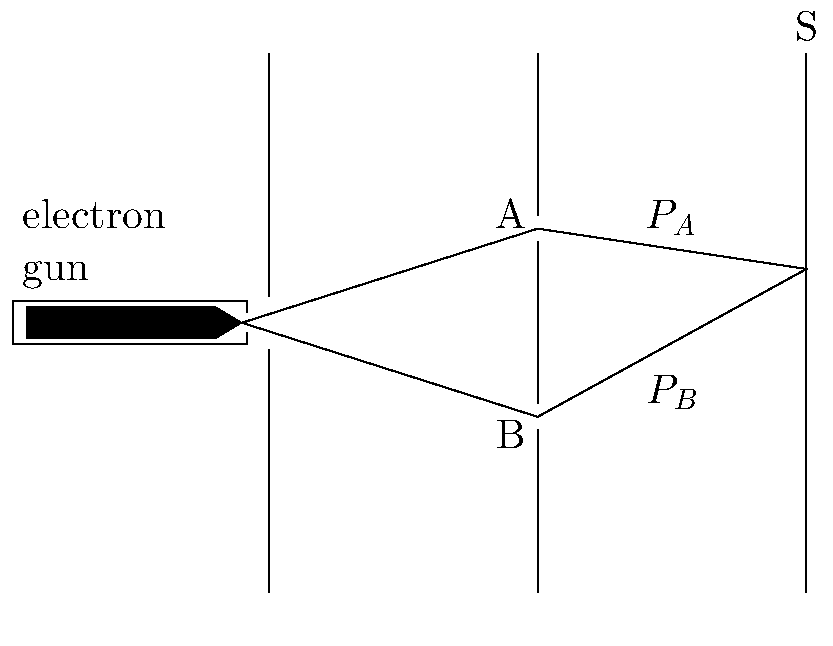
\includegraphics[width=.5\textwidth]{./Figure/Fig2-1.pdf}}
\end{figure}

Next, we generalize this approach as shown in Fig. \ref{Fig2-2}. Different from Fig. \ref{Fig2-1}, there is not just one screening shield, but many, and there are not two slits in each, but a large number (Fig. \ref{Fig2-2}a).

Depending on the way at each screen, many different combinations $c$ for passing through the slits are possible, each corresponding to an amplitude $a_c$, the total amplitude $a$ is given by $\sum _ { c } a _ { c }$. By increasing the number of screening layers and slits more and more, and finally reaching an infinite number, each screening layer will have many slits and finally will disappear. The interval between the gun and the screen will become a continuous space (Fig. \ref{Fig2-2}b), and depending on the “combination of slits” the path will mutate to an arbitrary path from the gun to the screen, and “the sum of all amplitudes of possible ways” will mutate to an integral over the paths, that is, the path integral. That is to say, the principle that “the amplitude corresponding to a transition from a starting point to an end point corresponds to an integral over the amplitudes of all possible paths linking these two points” can be regarded as the principle of quantum mechanics.

\begin{figure}[!b]
\begin{picture}(450,100)
\put(0,5){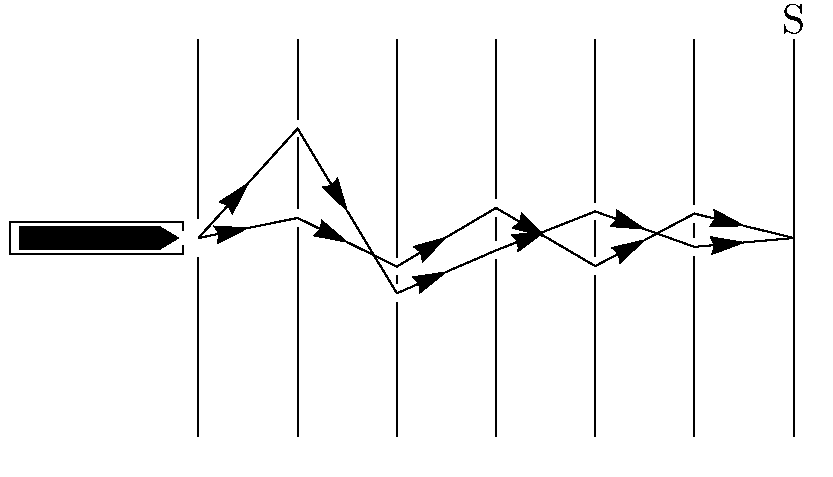
\includegraphics[width=.48\textwidth]{./Figure/Fig2-2a.pdf}}
\put(200,5){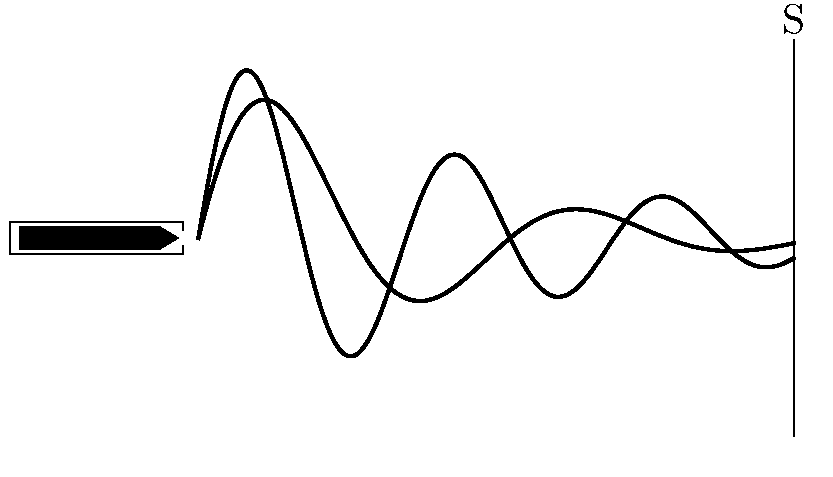
\includegraphics[width=.48\textwidth]{./Figure/Fig2-2b.pdf}}
\put(100,0){(a)}
\put(300,0){(b)}
\end{picture}
\caption{a, b. Generalization of the interference experiment of Fig. \ref{Fig2-1}. The number of screens and the number of slits in the screen is increased. }\label{Fig2-2}
\end{figure}

When considering quantum mechanics, one might have in mind the wave function, and the Schr\"{o}dinger equation of the wave function, all describing wave properties of the particle. It should be possible to link this description with the picture of the path integral described above by using the superposition principle of waves. However, it required the genius of Feynman to make this discovery.


We now turn to exact mathematics. We start from the Schr\"{o}dinger equation 
\be\label{eq2.1.1}
\begin{aligned} \mathrm { i } \hbar \frac { \partial \psi ( x , t ) } { \partial t } & = - \frac { \hbar ^ { 2 } } { 2 m } \frac { \mathrm { d } ^ { 2 } \psi ( x , t ) } { \mathrm { d } x ^ { 2 } } + V ( x ) \psi ( x , t ) \\ & = H \psi ( x , t ) \end{aligned}
\ee
For a moment, we restrict the motion of the particle to a one-dimensional space with space coordinate $x$. 

As shown in \eqref{eq1.1.3}, it is possible to integrate \eqref{eq2.1.1} formally
\be\label{eq2.1.2}
| \psi \left( t ^ { \prime } \right) \rangle = U \left( t ^ { \prime } , t \right) | \psi ( t ) \rangle = \mathrm { e } ^ { - ( 1 / \hbar ) H \left( t ^ { \prime } - t \right) } | \psi ( t ) \rangle
\ee
We choose $t' > t$. Equation \eqref{eq2.1.2} describes the time evolution of the state $| \psi ( t ) \rangle$ occurring at t through during the time $t'-t$, leading to the state $| \psi ( t' ) \rangle$. Not the wave function can be expressed with the path integral mentioned before, but the operator $U \left( t , t ^ { \prime } \right)$ describing the time evolution. In \eqref{eq2.1.2}, the label $x$ has been omitted intentionally, because $| \psi ( t ) \rangle$ should be regarded as a continuous infinite dimensional vector with components $\psi ( x , t )$ labelled by $x$, and $U \left( t ^ { \prime } , t \right)$ should be regarded as a matrix with components $U \left( x ^ { \prime } , t ^ { \prime } ; x , t \right)$. 

































































































\section{The Path Integral for Bosons}
\section{The Path Integral for Fermions}
\section{The Path Integral for the Gauge Field}
\section{The Path Integral for the Spin System}
\chapter{Symmetry Breaking and Phase Transition}
\section{Spontaneous Symmetry Breaking}
\section{The Goldstone Mode}
\section{Kosterlitz-Thouless Transition}
\section{Lattice Gauge Theory and the Confinement Problem}
\chapter{Simple Examples for the Application of Field Theory}
\section{The RPA Theory of a Coulomb Gas}
\section{The Bogoliubov Theory of Superfluidity}
\chapter{Problems Related to Superconductivity}\label{chap5}
\section{Superconductivity and Path Integrals}
\section{Macroscopic Quantum Effects and Dissipation: The Josephson Junction}
\section{The Superconductor-Insulator Phase Transition in Two Dimensions and the Quantum Vortices}
\chapter{Quantum Hall Liquid\\ and the Chern-Simons Gauge Field}
\section{Two-Dimensional Electron System}
\section{Effective Theory of a Quantum Hall Liquid}
\section{The Derivation of the Laughlin Wave Function}
\appendix

\chapter*{Appendix}
\chapter{Fourier Transformation}
\chapter{Functionals and the Variation Principle}\label{secapb}
\chapter{Quantum Statistical Mechanics}


\renewcommand{\bibname}{References}
\bibliographystyle{plain}
\bibliography{ref}


\end{document}  